\documentclass[a4paper,12pt]{article} %Dokumendiklassi defineerimine ja väljastatava teksti suuruse seadistamine       
\usepackage{graphicx} %Võimaldab teksti sees kasutada jooniseid
\usepackage[top=2.5cm, bottom=2.5cm, left=3cm, right=3cm]{geometry} %Määrab ära lehekülje suuruse
\usepackage{titlesec} %Vajalik pealkirjade modifitseerimiseks
\usepackage{longtable} %Vajalik pakett, et saaks teha üle ühe leheküljelisi tabeleid
\usepackage{multirow} %Vajalik, kui tahta tabelites mitut rida kokku panna
\usepackage{todonotes} %Vajalik, kui tahta lisada töösse todo märkmeid
\usepackage{url} %Vajalik, kui töös on kasutusel URL aadress. Sel juhul märkida URL tagi vahele ning LaTeX ei hakka seda lahti kompileerima eraldi käskudeks vms
\usepackage[figure,table,page,section]{totalcount} %Jooniste, tabelite, lehtede ja peatükkide arv
\usepackage{float} %Vajalik töös olevate tabelite ja jooniste vormistamiseks
\usepackage{longtable} %Korda tabeli päist uuel lehel
\usepackage{color,xcolor,colortbl}% Värvid
\definecolor{codegreen}{rgb}{0,0.6,0}
\definecolor{codegray}{rgb}{0.5,0.5,0.5}
\definecolor{codepurple}{rgb}{0.58,0,0.82}
\definecolor{rowgray}{gray}{0.85}
\usepackage{listings} %Koodi värvimiseks
\lstset{
    breaklines=true,
    frame=single
  }
\lstnewenvironment{SQL}
  {\lstset{
    breaklines=true,
    language=SQL,
    frame=single,
    framesep=5pt,
    basicstyle=\normalsize,
    %basicstyle=\footnotesize,
    commentstyle=\color{codegreen},
    keywordstyle=\color{blue},
    numberstyle=\tiny\color{codegray},
    stringstyle=\color{codepurple},
    keepspaces=true,                 
    numbers=left,                    
    numbersep=2pt,                  
    showspaces=false,                
    showstringspaces=false,
    showtabs=false,                  
    tabsize=2
  }}
  {}

\usepackage[estonian]{babel} %Eestikeelsete tähtede kasutamise võimalus
\usepackage[T1]{fontenc} %Vajalik vene ja eesti  keelsete tähtede kasutamiseks
\usepackage[utf8]{inputenc} %UTF8 dekodeerimise kasutamine

\addto\captionsestonian{\def\refname{\centerline{Kasutatud kirjandus}}} %Muudab viidete nime kasutatud kirjanduseks ning paigutab lehe keskele
\addto\captionsestonian{\def\listfigurename{\centerline{Jooniste loetelu}}} %Muudab jooniste nimekirja nime jooniste loeteluks ning paigutab selle lehe keskele
\addto\captionsestonian{\def\listtablename{\centerline{Tabelite loetelu}}} %Muudab tabelite nimekirja nime tabelite loeteluks ning paigutab selle lehe keskele
\addto\captionsestonian{\def\contentsname{\centerline{Sisukord}}}
	
\usepackage{tocloft} %Selleks, et modifitseerida sisukorda
\usepackage{amssymb} %Erisümbolid
\renewcommand{\labelitemi}{\tiny$\blacksquare$} %Loetelude ees kuvatakse ruudukesi

\usepackage{caption} %Vajalik tabelite ja jooniste pealkirjastamisel
\captionsetup{labelsep=period} %Lisab tabeli või joonise nime lõppu punkti

\usepackage{verbatimbox} %Koodi kuvamine lehe keskel

\titlelabel{\thetitle.\quad} %Lisab pealkirjade lõppu punkti

\usepackage{times} %Tekst on Times tüüpi
\usepackage{fancyhdr} %Võimaldab kasutada päiseid ja jaluseid
\setlength{\parindent}{0cm} %Lõigu taane on seatud nulliks
\usepackage{setspace} %Vajalik teksti vahede seadistamiseks
\onehalfspacing %Ridade vahel on 1,5 tähe kõrgusest
\setlength{\parskip}{12pt}%Lõiguvahe

\usepackage{hyperref} %Muudab lingid klikitavaks

\hyphenation{} %Ebakorrektse poolitamise parandamine kujul: \hyphenation{üliõpilas-kood lehe-küljed}

\titleformat{\section}{\normalfont\Large\bfseries}{\thesection}{16pt}{} %Sectioni tekstisuurus
\titleformat{\subsection}{\normalfont\large\bfseries}{\thesubsection}{14pt}{} %Subsectioni tekstisuurus
\titleformat{\subsubsection}{\normalfont\normalsize\bfseries}{\thesubsubsection}{12pt}{} %Subsubsectioni tekstisuurus

%\titlespacing*{\section}{0pt}{44pt}{18pt} %Sectioni ees, ülal ja all olev ruum
\titlespacing*{\subsection}{0pt}{24pt}{12pt} %Subsectioni  ees, ülal ja all olev ruum
\titlespacing*{\subsubsection}{0pt}{12pt}{12pt} %Subsubsectioni ees, ülal ja all olev ruum

\newcommand{\sectionbreak}{\clearpage} % Iga section algab uuelt lehelt

\begin{document}

%------------------------------TIITELLEHT---------------------------------
\thispagestyle{fancy} %Leht sisaldab päist ja jalust
\renewcommand{\headrulewidth}{0pt} %Eemaldab päisest horisontaalse joone
\renewcommand{\footrulewidth}{0pt} %Eemaldab jalusest horisontaalse joone
\headheight = 60pt %Paneb paika päise laiuse (vastavalt kompilaatori soovitusele)
\footskip = 9pt %Jaluse ruum
\headsep = 0pt %Vähendab päise ja teksti vahelise kauguse nullini

\chead{ %Paigutab järgneva teksti päises keskele
 \textsc{\begin{Large} %Tekst suurtähtedega ja suuremaks
	tallinna tehnikaülikool\\
	\end{Large} }
	Infotehnoloogia teaduskond\\
	Informaatika instituut\\
	Infosüsteemide õppetool
}
\vspace*{140pt} %Tekitab lehe alguse ja teksti vahele tühja ala vastava laiusega

\begin{center} %Tekst keskele
\begin{LARGE}
PostgreSQL-i põhise meta-andmetega juhitavate veebirakenduste kiirprogrammeerimiskeskkonna projekteerimine ja realiseerimine\\[20pt]
\end{LARGE}
Magistritöö\\[60pt]
\end{center}

\begin{flushright} %Joondab teksti paremale
\begin{tabular}{p{80pt}p{100pt}}
Üliõpilane:&Rait Raidma\\
Üliõpilaskood:&143682IAPM\\
Juhendaja:&dotsent Erki Eessaar\\
\end{tabular}
\end{flushright}

\cfoot{Tallinn\\2016} %Lisab asukoha ja kuupäeva jalusesse
\pagebreak %Lehe lõpp

%---------------------------AUTORIDEKLARATSIOON-------------------------
\section*{\begin{center}
 Autorideklaratsioon
\end{center}}

Kinnitan, et olen koostanud antud lõputöö iseseisvalt  ning seda ei ole kellegi teise poolt varem kaitsmisele esitatud. Kõik töö koostamisel kasutatud teiste autorite tööd, olulised seisukohad, kirjandusallikatest ja mujalt pärinevad andmed on töös viidatud.\\[50pt]

\begin{center}
\begin{tabular}{cc}
......................................................&......................................................\\
\textit{(kuupäev)}&\textit{(allkiri)}\\
\end{tabular}
\end{center}

\pagebreak

%---------------------------ANNOTATSIOON---------------------------------
\section*{\begin{center}
Annotatsioon
\end{center}}

Lõputöö on kirjutatud eesti keeles ning sisaldab teksti \totalpages{} leheküljel, \totalsections{} peatükki, \totalfigures{} joonist, \totaltables{} tabelit.
\pagebreak
%-----------------------------ABSTRACT-----------------------------------
\section*{\begin{center}
Abstract
\end{center}}
The thesis is in estonian and contains \totalpages{} pages of text, \totalsections{} chapters, \totalfigures{} figures, \totaltables{} tables.
\pagebreak
%---------------------LÜHENDITE JA MÕISTETE SÕNASTIK---------------------
\section*{\begin{center}
Lühendite ja mõistete sõnastik
\end{center}}
\begin{tabular}{p{3cm}p{11cm}} %Tabel, mille esimese lahtri laius on 3cm.
SQL&\textit{Structured Query Language}, struktureeritud andmebaasikeel andmete käitlemiseks, õiguste jagamiseks ning andmebaasiobjektide haldamiseks\\
FSF&\textit{Free Software Foundation}, MTÜ, mis propageerib arvuti kasutajate vabadust ja kaitseb vaba tarkvara kasutajate õigusi\\
OSI&\textit{Open Source Initiative}, Organisatsioon, mis propageerib avatud lähtekoodiga tarkvara\\
Juurutama&\textit{Deploy}, Tarkvara või riistvara töölepanekuga seotud protsesside - installeerimine, konfigureerimine, käitamine, testimine - läbimine \cite{Vallaste}\\
CRUD&\textit{Create Read Update Delete}, Lühend, mis tähistab andmetega manipuleerimise nelja põhitegevust: loomine, lugemine, muutmine ja kustutamine\\
Meta-andmed&Andmed andmete kohta\\
\end{tabular}
\pagebreak
%----------------------------SISUKORD----------------------------------
\tableofcontents
\newpage
%----------------------JOONISTE NIMEKIRI-------------------------------
\listoffigures
\pagebreak
%----------------------TABELITE NIMEKIRI---------------------------------
\listoftables
\pagebreak
%-----------------------------SISSEJUHATUS------------------------------- 
\section{Sissejuhatus}
\label{Sissejuhatus} %Võimaldab pealkirjale viidata \ref käsuga
\subsection{Taust ja probleem}
TTÜ-s õpetatava aine ``Andmebaasid II'' raames tuleb üliõpilastel ühe õpiväljundina luua andmebaas koos seda kasutava rakendusega, kus rakendus suhtleb andmebaasiga läbi avaliku andmebaasiliidese. Andmebaasi loomiseks võib kasutada andmebaasisüsteeme PostgreSQL \cite{PostgreSQL} ja Oracle \cite{Oracle_DB}. Juhul, kui andmebaas on loodud Oracle andmebaasisüsteemi abil, siis on üliõpilastel rakenduse loomiseks võimalus kasutada Oracle APEX-it \cite{Oracle_APEX}. PostgreSQL andmabaasisüsteemiga loodud andmebaasi korral tuleb rakendus programmeerida kasutades PHP-d \cite{PHP}. See tähendab, et üliõpilane ei saa keskenduda täielikult andmebaasi täiustamisele vaid peab tegelema ka lisaprogrammeerimisega, mis olenevalt eelnevast kogemusest võib võtta rohekm või vähem aega. Töö tulemusena valmiva prototüübi abil peaks üliõpilastel olema lihtsam luua näidisrakendusi, mis kasutavad andmebaasisüsteemina PostgreSQL-i.\par
Töö valmis 2016. aasta kevadel Tallinna Tehnikaülikoolis.
\subsection{Ülesande püstitus}
Antud töö eesmärgiks on uurida, kuidas luua PostgreSQL andmebaasi põhjal meta-andmetega juhutavat veebipõhist rakenduste kiirprogrammeerimiskeskkonda ning see realiseerida. Loodav süsteem peab toetama PostgreSQL 9.4 ja PHP 5.5.0.
Töö tulem avaldatakse avatud lähtekoodi litsentsi all. \par
Loodava süsteemi abil peavad kasutajad saama valida, millise andmebaasi põhjal nad soovivad enda rakenduse luua. Kasutades andmebaasi avalikku liidest peab olema võimalik luua lehekülgi, lisada neile raporteid, vorme ning navigeerida erinevate lehtede vahel. Sisselogimine peab olema võimalik, kasutades sama kasutajanime ja parooli, mis on kasutusel andmebaasisüsteemis.
\subsection{Metoodika}
Süsteemi realiseerimiseks kasutatakse serveri poole pealt andmebaasisüsteemi PostgreSQL 9.4 \cite{PostgreSQL}, programmeerimiskeelt PHP 5.5.0 \cite{PHP}, PHP raamistikku Slim 3.3.0 \cite{SlimFW}. Kliendi poole realiseerimiseks kasutatakse lisaks HTML-le ja CSS-le ka AngularJS 1.4 \cite{AngularJS} ja Bootstrap 3 \cite{Bootstrap}.
Selleks, et loodud süsteemi oleks ka teistel lihtne üles seada ning kasutada, loon Vagrant-i \cite{Vagrant} abil virtuaalmasina, kus on eelnevalt installitud kogu vajalik tarkvara süsteemi arendamiseks ja testimiseks. Javascripti koodi testimiseks kasutan Karma 0.13 \cite{karma} ja Jasmine 2.3 \cite{Jasmine}. PHP koodi testimiseks kasutan PHPUnit 4.8 \cite{PHPUnit} ja Mockery 0.9 \cite{Mockery}. Testide automaatseks jooksutamiseks ning koodi juurutamiseks (\textit{deploy}) kasutan TravisCI \cite{TravisCI} keskkonda. Koodi ennast hoitakse GitHub-i \cite{GitHub} koodihoidlas.
\subsection{Ülevaade tööst}
TODO
\pagebreak

\section{Teoreetiline taust}
\subsection{Andmebaasi avalik liides}
Liides on sõltumatute süsteemide vaheline leping, kus on kirjeldatud, millisel viisil saab üks süsteem teisega suhelda.
Andmebaasis saab liideseid kirjeldada rutiinidena ja vaadetena.

\begin{figure}[H]
\begin{center}
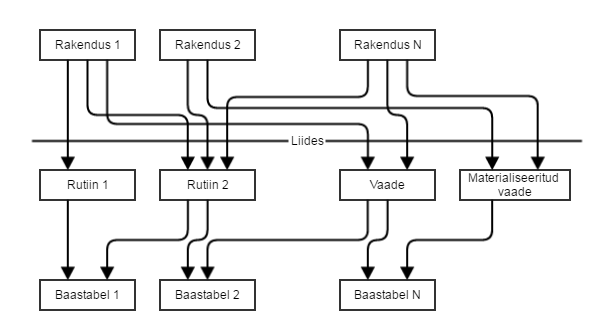
\includegraphics[bb=0 0 606 330,scale=0.6]{./diagrams/db-interface.png}
\caption{Andmebaasi avalik liides}
\end{center}
\end{figure}

\subsubsection{Vaadete kasutamise eelised}
\begin{itemize}
\item Võimaldavad igale rakendusele saab luua spetsiifilise vaate andmetest, ilma et oleks vaja teha muudatusi andmemudelis.
\item Võimaldavad vähendada rakenduse koodi ja andmemudeli vahelist sidusust.
See võimaldab teha muudatusi andmemudelis, ilma et olemasolev rakendus katki läheks.
\item Neile saab anda rakenduse-spetsiifilised veerunimed, andmetüübid ja pikkused, mis võimaldab otse andmete sidumist rakenduses kasutatavate mudelitega.
\item Võimaldavad jõustada andmete turvamist. Erinevatele kasutajagruppidele saab kuvada andmeid erineval kujul, nii et kasutaja näeb üksnes neid andmeid, mida ta on volitatud nägema. PostgreSQL andmebaasisüsteemis tuleks lisaks kasutada \textit{WITH (security\_barrier)} lisatingimust. See takistab peidetud ridade kuvamist ka juhul, kui kasutatakse kuritahtlikult valitud funktsioone ja operaatoreid, et näha varjatud infot \cite{PostgreSQLRulesAndPrivileges}
\item Võimaldavad pärida andmeid erinevatest tabelitest ja andmebaasidest, peites kasutajate eest päringu tegeliku keerukuse. Vaate koostamiseks vajalik päring on eelnevalt kompilleeritud ja optimiseeritud, et tagada parem jõudlus. Vaated kasutavad päringu täitmisel baastabelitele loodud indekseid.
\item Võimaldavad varjata rakenduse eest baastabelites olevaid disaini -ja andmevigasid, andes lisaaega nende parandamiseks.
\item Võimaldavad kuvada samu andmeid erineval kujul ühendatuna, kasvõi nt XML-na või JSON-na.
\item Läbi vaadete, mis vastavad teatud tingimustele, on võimalik teha andmemuudatusi baastabelites, kui realiseerida INSTEAD OF triggerid.
\end{itemize}
\cite[lk 172-173]{BuildingTheAgileDatabase}

\subsubsection{Rutiinide kasutamise eelised}
\begin{itemize}
\item Üle võrgu saadetavate andmete ja SQL koodi hulk hoitakse minimaalsena, mille tulemusel suureneb rakenduse jõudlus.
\item Rutiinide kood on andmebaasi serveris eelnevalt kompilleeritud ja optimiseeritud, suurendades rutiini täitmise efektiivsust.
\item Andmetöötluse jaoks kasutatakse andmebaasiserveri jõudlust, mitte rakendusserveri ega kliendi masina oma.
\item Rutiinis olevat SQL koodi on lihtsam testida ja optimiseerida, kui rakendusse sisse kirjutatud SQL-i.
\item Rutiinide käivitusõiguste abil saab piirata ligipääsu teatud rollidele ning suurendada seeläbi turvalisust.
\item Rutiinis käivitatavad laused tehakse ühe transaktsiooni jooksul. See aitab vältida osalisi andmemuudatusi, kus üks osa muudatustest läks läbi, teine osa aga mitte.
\end{itemize}
\cite[lk 179, 195]{BuildingTheAgileDatabase}

\subsection{Ühendumine teiste andmebaasidega}
Loodava süsteemi üheks tingimuseks on, et selle abil peab saama luua rakendusi erinevate andmebaaside põhjal. PostgreSQL andmebaasisüsteemis pole realiseeritud andmebaaside vahelisi viitasid ning seetõttu ei saa koostada päringuid kujul:
\begin{SQL}
select * from other_db_name.schema_name.table_name;
\end{SQL}
Eelnev päring annab tulemuseks veateate:
\begin{lstlisting}
ERROR:  cross-database references are not implemented: "other_db_name.schema_name.table_name"
\end{lstlisting}
Selleks, et ühenduda väliste PostgreSQL andmebaasidega, tuleb kasutada kas dblink või postgres\_fdw moodulit.
\subsubsection{dblink}
\label{dblink}
Mooduli installeerimine:
\begin{SQL}
CREATE EXTENSION IF NOT EXISTS dblink;
\end{SQL}
Andmete küsimiseks välisest andmebaasist tuleb ette anda andmebaasi nimi, kasutaja ja parool ning lause, mida käivitada soovitakse. Päring käivitatakse välises andmebaasis. Päringuks võib olla iga SQL lause, mis tagastab read.\cite{PostgreSQLdblink} Allpool on toodud näide päringu koostamisest dblink mooduli abil.
\begin{SQL}
SELECT schema_name, owner_id
FROM dblink(
  'dbname=external_database_name user=external_database_user password=external_database_user_password',
  'SELECT upper(nspname), nspowner FROM pg_catalog.pg_namespace;'
) AS (
  schema_name varchar,
  owner_id int
);
\end{SQL}

\subsubsection{postgres\_fdw}
Selle mooduli poolt pakutav funktsionaalsus kattub suurel määral \textit{dblink} \ref{dblink} mooduli funktsionaalsusega, kuid pakub standardsemat süntaksit päringute koostamiseks ning võib kohati edestada jõudluse poolest. Küll aga pole võimalik välja kutsuda välises andmebaasis olevaid funktsioone.
\cite{PostgreSQLfdw}

\subsubsection{Mooduli valik}
Kuna loodav süsteem peab suutma välja kutsuda välistes andmebaasides olevaid funktsioone, siis pole tuleb kasutada \textit{dblink} \ref{dblink} moodulit.

\subsection{Uue süsteemi visioon}
Eesmärk on luua lihtsasti kasutatav veebipõhine süsteem, mille abil saaks kiiresti luua teisi veebipõhiseid rakendusi. Loodavates rakendustes peab andmete pärimine, lisamine, muutmine ning kustutamine käima läbi andmebaasi avaliku liidese. Kogu vajalik info rakenduse loomiseks tuleb hoida andmebaasis.
\subsection{Eksisteerivate programmide analüüs}
\subsubsection{Oracle Application Express (APEX)}
Oracle APEX on veebipõhine rakendus loomaks kiirelt ja lihtsalt teisi veebipõhiseid rakendusi. Kogu süsteem on juhitav andmebaasis hoitavate metaandmetega. APEX kasutab tööks Oracle anembaasisüsteemi.\par
APEX (v 5.0.3.00.03) koosneb neljast põhiosast:
\begin{itemize}
\item Application Builder - Võimaldab luua ja hallata uusi rakendusi. Rakendused koosnevad lehtedest. Lehed omakorda sisaldavad regioone. Regioonides võib kuvada raporteid, graafikuid, vorme jpm. Regioonid sisaldavad komponente, mille abil on võimalik kasutajalt infot küsida ning seda esitada. Lisaks on võimalik nähe lehtede statistikat ning hallata seadeid.
\item SQL Workshop - Võimaldab näha ja hallata andmebaasiobjekte, jooksutada päringuid, importida/exportida anmebaasis olevaid andmeid, koostada pärngkuid graafilise liidese abil, luua RESTful liideseid jpm.
\item Team Development - Tööde- ja vigadehaldus süsteem. Võimaldab arendajatel ülesandeid planeerida ja hallata.
\item Packaged Apps - Galerii näidisrakendustest, mida on võimalik kohe kasutamiseks installeerida.
\end{itemize}
\cite{Oracle_APEX}
\subsubsection{NuBuilder}
NuBuilder on veebipõhine arendusplatvorm loomaks veebipõhiseid rakendusi. Lehtede kirjeldused (sh PHP, JS ja SQL päringud) hoitakse andmebaasis, mis muudab rakenduse varundamise lihtsaks.\par
NuBuilder on kirjutatud PHP-s ning andmeid hoitakse MySQL andmabaasisüsteemis. Tabelite põhjal on võimalik luua lihtsaid CRUD vorme, kus on võimalik tabelis olevaid andmeid lugeda, lisada, muuta ja kustutada. SQL päringute põhjal on võimalik luua raporteid, mida arendaja saab veebiliidese kaudu disainida.
Oma kodulehel väidavad nad, et tegu on \textit{Open Source} tarkvaraga ning lähtekood on avalikult üleval \cite{nuBuilderGitHub}, kuid kusagil pole mainitud, millise \textit{Open Source} litsentsi alt on tarkvara välja antud.\par
Koodi puhul täheldasin mitut puudujääki:
\begin{itemize}
\item Failid on kehvasti struktureeritud - php, js, png ja gif failid on kõik koos ühes kaustas.
\item PHP ja HTML on kirjutatud läbisegi, mis teeb disaini muutmise keeruliseks.
\item Kasutatakse \$GLOBALS muutujat - see raskendab arusaamist, kus võidakse muutujale programmi töö ajal väärtusi omistada.
\item Funktsioonid on liiga pikad - paljud funktsioonid täidavad korraga liiga palju ülesandeid ja seetõtu on raskendatud nendest arusaamine.
\end{itemize}
\cite{nuBuilder}
\subsubsection{Xataface}
Xataface on programm, millega saab tabelite põhjal genereerida vorme ja kuvasid. Pärast genereerimist tuleb loodud failid serverisse üles laadida. Lehtede konfigureerimine toimub INI failide abil.\cite{Xataface}\par
Xataface on avatud lähtekoodiga ning antud välja GPL litsentsi all. Programm on kirjutatud PHP-s \cite{PHP} ning andmebaasina kasutatakse MySQL-i \cite{MySQL}.\par
Kasutatud on palju väliseid teeke. Programmil on üks põhiline arendaja ning igapäevast arendustööd ei toimu. \cite{XatafaceGitHub}
\subsection{Täpsustunud ülesande püstitus}
\subsection{Kasutatavad tehnoloogiad}
\subsubsection{Vagrant 1.8.1}
Vagrant on käsureaprogramm, millega saab hallata virtuaalmasina elutsüklit. Vagrant isoleerib programmilised sõltuvused ja nende konfiguratsioonid ühtsesse eraldiseisvasse keskkonda. Keskkonna konfigureerimiseks saab kasutada käsurea käsklusi, \textit{Ansible}-t \cite{Ansible}, \textit{Puppet}-it \cite{Puppet}, \textit{Chef}-i \cite{Chef}, \textit{Docker}-it \cite{Docker} ja \textit{Salt}-i \cite{Salt}. Tänu Vagrantile saavad kõik luua endale täpselt ühesuguse keskkonna, kus programme jooksutada, vähendades võimalust, et ühes arvutis programm jookseb, teises aga mitte. \cite{Why_Vagrant}
\subsubsection{Apache HTTP server}
Apache HTTP server on avatud lähtekoodiga HTTP veebiserver.\cite{About_Apache_HTTPD}
\subsubsection{PHP 5.5.3}
PHP \textit{(PHP: Hypertext Preprocessor)} on avatud lähtekoodiga skriptimiskeel, mis on peamiselt mõeldud veebiprogrammeerimiseks. \cite{What_Is_PHP} PHP koodi protsessitakse PHP interpretaatori abil. Üldjuhul kasutatakse interpreteerimiseks \textit{Zend Engine}-t, kuid PHP-d võimalik jooksutada kasutada ka \textit{HHVM}-i \cite{HHVM} abil. PHP toetab erinevaid operatsioonisüsteeme, sealhulgas Windows-i erinevaid versioone ja Linuxi erinevaid distributsioone.
\subsubsection{Postgresql 9.4}
PostgreSQL on avatud lähtekoodiga objekt-relatsiooniline andmebaasisüsteem, mis vastab täielikult \textit{ACID} nõuetele. See toetab \textit{foreign key}-sid, \textit{join}-e, \textit{view}-sid, \textit{trigger}-eid ja salvestatud protseduure. PostgreSQL toetab erinevaid operatsioonisüsteeme, sealhulgas Windows-i erinevaid versioone ja Linuxi erinevaid distributsioone.
\cite{PostgreSQL_About}
\subsubsection{Javascript}
\subsubsection{AngularJS}
\subsubsection{Bootstrap}
\subsection{Litsents}
\subsubsection{Free Software}
\textit{Free Software} (Vaba tarkvara) tähendab, et kasutajatel on vabadus tarkvara jooksutada, kopeerida, levitada, uurida, muuta ja täiustada. Seega \textit{Free Software} on kasutaja vabaduse, mitte hinna küsimus. \par
Tarkvara on \textit{Free Software}, kui selle kasutajate jaoks on täidetud neli olulist kriteeriumit:
\begin{itemize}
\item Vabadus 0: jooksutada programmi oma suva järgi, ükskõik mis eesmärgil
\item Vabadus 1: uurida, kuidas programm töötab ja seda muuta (eeldab ligipääsu lähtekoodile)
\item Vabadus 2: levitada antud tarkvara
\item Vabadus 3: levitada antud tarkvara muudetud kujul (eeldab ligipääsu lähtekoodile)
\end{itemize}
Vabadus levitada (vabadused 2 ja 3) tähendab vabadust jagada antud tarkvara muudetud või muutmata kujul kas tasu eest või tasuta - selleks ei pea kelleltki luba küsima. Küll aga peab jagatav koopia sisaldama nii lähtekoodi kui ka käivitatavat programmi (kui programmeerimiskeel toetab seda võimalust)\par
\textit{Free Software} ei tähenda, et tegu ei võiks olla kommertstarkvaraga. \textit{Free Software} võib omandada tasuta või raha eest. Vaatamata sellele, kuidas koopia antud tarkvarast omandati,  jääb omandajale vabadus antud tarkvara jagada, muuta ja müüa.
\cite{GNU_Free_SW}
\subsubsection{Open Source}
\textit{Open Source} (Avatud lähtekood) ei tähanda ainult ligipääsu lähtekoodile. Tarkvara levitamisel peab lätuma järgmistest reeglitest:
\begin{enumerate}
\item Vaba jagamine - Litsents ei tohi piirata ühtegi osapoolt tarkvara müümast või jagamast.
\item Lähtekood -  Tarkvara peab sisaldama lähtekoodi ning lähtekoodi ja kompileeritud koodi jagamine peab olema lubatud. Kui tarkvara ei jagata koos lähtekoodiga, peab lähtekood olema mujalt mõistliku vaevaga kättesaadav.
\item Tuletatud tarkvara - Litsents peab lubama muudatusi ja tuletatud tarkvara ning peab lubama nende jagamist samadel litsentsitingimustel.
\item Autori lähtekoodi terviklikkus - Litsents võib keelata muudetud lähtekoodi jagamist üksnes siis, kui on lubatud jagada paikefaile (\textit{patch file}), et muuta programmi lähtekoodi selle loomise mingis järgus (\textit{build time}). Litsents peab selgelt lubama muudetud lähtekoodiga tarkvara jagamist. Litsents võib nõuda, et tuletatud tarkvara kannaksid teist nime või versiooninumbrit, kui originaaltarkvara.
\item Isikute või gruppide diskrimineerimiskeeld - Litsents ei tohi diskrimineerida ühtegi isikut või isikute gruppi.
\item Tegevusvaldkonna diskrimineerimiskeeld - Litsents ei tohi piirata ühtegi konktreetset tegevusvaldkonda.
\item Litsentsi jagamine - Programmile sätestatud õigused kehtivad kõigile, kellele programm on jagatud, ilma, et osapooled vajaksid täiendavat litsentsi.
\item Litsents ei tohi olla tootespetsiifiline - Programile sätestatud õigused ei tohi sõltuda sellest, kas programm kuulub mõne teise programmi koosseisu.
\item Litsents ei tohi piirata teisi tarkvarasid - Litsents ei tohi panna piiranguid teistele tarkvaradele, mida jagatakse koos antud tarkvaraga.
\item Litsents peab olema tehnoloogiliselt neutraalne - Ükski klausel ei tohi viidata konkreetsele tehnoloogiale, stiilile või liidesele.
\end{enumerate}
\cite{Open_Source_Def}
\subsubsection{\textit{Free Software} ja \textit{Open Source} võrdlus}
\textit{Open Source} kriteeriumid on veidi vabamad kui \textit{Free Software} omad. Kõik eksisteerivad \textit{Free Software} programmid kvalifitseeruvad \textit{Open Source} tarkvara alla. Enamik \textit{Open Source} tarkvarast on \textit{Free Software}, kuid leidub ka erandeid.
\cite{OS_VS_FS}
\begin{itemize}
\item Mõlemad nimed ei väljenda täpselt seda, mida nende all tegelikult on mõeldud.
\item Mõlemad lubavad tarkvara jagada tasuta või seda müüa.
\item \textit{Open Source} kriteeriumid kehtivad ainult lähtekoodile, mitte aga kompilleeritud programmile.
\end{itemize}
\subsubsection{Litsentsi valik}
Üheks töö eesmärgiks oli avaldada loodava prototüübi lähtekood avatud tarkvarana. Olemasolevaid litsentse on väga palju. Selleks, et valida välja litsents, mille all avaldada loodav tarkvara, leian esiteks populaarseimad litsentsid ning võdlen neid omavahel.
GitHub-i poolt avaldatud statistika kohaselt on populaarseimad litsentsid: MIT (44,69\%), GPLv2 (12,96\%), Apache (11,19\%) ja GPLv3 (8,88\%). \cite{GitHub_Opensource_Licence_Usage}\par
Kõik eelpool nimetatud litsentsid täidavad nii \textit{Open Source} kui ka \textit{Free Software} tingimusi. Tabelis \ref{table_litsentside_vordlus} on välja toodud litsentside võrdlus.

\begin{table}[H]%[!htb]
\begin{center}
\begin{tabular}{|p{3cm}|p{4cm}|p{4cm}|p{4cm}|}
\hline
\rowcolor{rowgray}
 & Nõutud & Lubatud & Keelatud \\ \hline
MIT & Litsents ja copyright märge & Kaubanduslik kasutamine & Võtta vastutusele \\
 &  & Jagamine &  \\
 &  & Muutmine &  \\
 &  & Privaatne kasutamine &  \\ \hline
Apache \newline License 2.0 & Litsents ja copyright märge & Kaubanduslik kasutamine & Võtta vastutusele \\
 & Teavitus muudatustest & Jagamine & Kasutada kaubamärki \\
 &  & Muutmine &  \\
 &  & Patendi kasutamine &  \\
 &  & Privaatne kasutamine &  \\ \hline
GNU GPLv3 & Lähtekoodi avaldamine & Kaubanduslik kasutamine & Võtta vastutusele \\
GNU GPLv2 & Litsents ja copyright märge & Jagamine &  \\
 & Sama litsents & Muutmine &  \\
 & Teavitus muudatustest & Patendi kasutamine &  \\
 &  & Privaatne kasutamine & \\ \hline
\end{tabular}
\caption{Litsentside võrdlus}
\label{table_litsentside_vordlus}
\cite{Licences}
\end{center}
\end{table}
Valitud sai MIT litsents, kuna see seab kasutajatele kõige vähem piiranguid ning arendajale kõige vähem kohustusi.
\section{Süsteemi analüüs}
\subsection{Tegutsejad}
\begin{itemize}
\item Administraator.
\item Kasutaja.
\end{itemize}
\subsection{Terviksüsteemi tükeldus allsüsteemideks}
\subsubsection{Pädevusalad}
\begin{itemize}
\item Administraatori pädevusala.
\item Kasutaja pädevusala.
\end{itemize}
Administraatori pädevusala kasutab kõiki allsüsteeme.\par
Kasutaja pädevusala kasutab ainult rakenduse allsüsteemi.
\subsubsection{Funktsionaalsed allsüsteemid}
\begin{itemize}
\item Rakenduse funktsionaalne allsüsteem.
\item Rakenduste funktsionaalne allsüsteem.
\item Lehtede funktsionaalne allsüsteem.
\item Regioonide funktsionaalne allsüsteem.
\item Navigatsioonide funktsionaalne allsüsteem.
\item Mallide funktsionaalne allsüsteem.
\end{itemize}
Antud töös ei realiseerita mallide funktsionaalset allsüsteemi.
\subsubsection{Registrid}
\begin{itemize}
\item Andmebaasiobjektide register.
\item Rakenduste register.
\item Lehtede register.
\item Regioonide register.
\item Navigatsioonide register.
\item Mallide register.
\end{itemize}

\subsection{Rakenduse funktsionaalne allsüsteem}
\subsubsection{Eesmärgid}
\begin{itemize}
\item Võimaldada administraatoril ja kasutajal kasutada loodud rakendust.
\end{itemize}
\subsubsection{Allsüsteemi poolt kasutatavad registrid}
Allsüsteem ei teeninda ühtegi registrit.\par
Allsüsteem kasutab andmebaasiobjektide registrit, rakenduste registrit, lehtede registrit, regioonide registrit, navigatsioonide registrit, mallide registrit.
\subsubsection{Allsüsteemi kasutusjuhtude eskiismudel}
Järgnevalt on esitatud rakenduse funktsionaalse allsüsteemi kasutusjuhtude eskiismudel ja seal esitatud tekstikirjeldused kõrgtaseme formaadis.
\begin{figure}[H]
\begin{center}
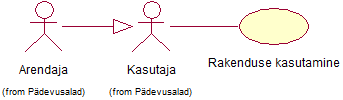
\includegraphics[bb=0 0 432 301,scale=1]{./diagrams/application-subsystem-use-case-digram.png}
\caption{Rakenduse funktsionaalse allsüsteemi kasutusjuhtude eskiismudel}
\end{center}
\end{figure}

\underline{\textbf{Kasutusjuht:} Rakenduse kasutamine}
\par
\textbf{Tegutsejad:} Kasutaja
\par
\textbf{Kirjeldus:} Kasutaja saab kasutada loodud rakendust.
\par

\underline{\textbf{Kasutusjuht:} Rakenduse kasutaja identifitseerimine}
\par
\textbf{Tegutsejad:} Kasutaja
\par
\textbf{Kirjeldus:} Kui rakenduses kuvatav lehekülg nõuab, et kasutaja on autenditud, siis kuvatakse kasutajale autentimisvorm, kus küsitakse kasutajanime ja parooli. Kui kasutaja poolt sisestatud kasutajanimi ja parool on korrektsed, siis lubatakse kasutajal näha kaitstud lehekülgi. Kasutaja peab sessiooni jooksul autentima ainult ühe korra.
\par

\underline{\textbf{Kasutusjuht:} Lehe vaatamine}
\par
\textbf{Tegutsejad:} Kasutaja
\par
\textbf{Kirjeldus:} Kasutaja näeb lehel loodud regioonide sisu. Lehel võidakse kuvada navigatsioone, raporteid, vorme ja HTML teksti.
\par

\underline{\textbf{Kasutusjuht:} Lehtede vahel navigeerimine}
\par
\textbf{Tegutsejad:} Kasutaja
\par
\textbf{Kirjeldus:} Kasutaja saab navigeerida erinevate lehtede vahel vajutades navigatsioonil olevatele linkidele.
\par

\underline{\textbf{Kasutusjuht:} Vormi esitamine}
\par
\textbf{Tegutsejad:} Kasutaja
\par
\textbf{Kirjeldus:} Kasutajale kuvatakse vorm, mis võib olla juba eelnevalt täidetud. Kasutaja sisestab ormi väljadesse andmed ning saadab need vormi esitamisega töötlemisse.
\par

\subsection{Rakenduste funktsionaalne allsüsteem}
\subsubsection{Eesmärgid}
\begin{itemize}
\item Võimaldada administraatoril saada ülevaade loodud rakendustest.
\item Võimaldada administraatoril luua uus rakendus.
\item Võimaldada administraatoril muuta olemasolevate rakenduste seadeid.
\item Võimaldada administraatoril kustutada olemasolevaid rakendusi.
\end{itemize}
\subsubsection{Allsüsteemi poolt kasutatavad registrid}
Allsüsteem teenindab rakenduste registrit.\par
Allsüsteem kasutab andmebaasiobjektide registrit.
\subsubsection{Allsüsteemi kasutusjuhtude eskiismudel}
Järgnevalt on esitatud rakenduste funktsionaalse allsüsteemi kasutusjuhtude eskiismudel ja seal esitatud tekstikirjeldused kõrgtaseme formaadis.
\begin{figure}[H]
\begin{center}
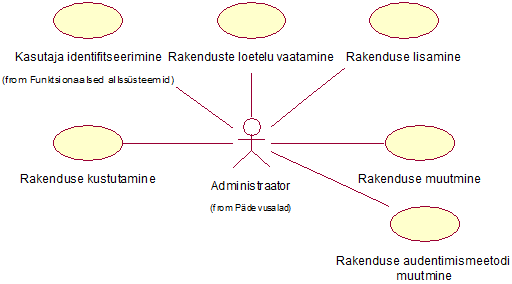
\includegraphics[bb=0 0 494 223,scale=1]{./diagrams/applications-subsystem-use-case-digram.png}
\caption{Rakenduste funktsionaalse allsüsteemi kasutusjuhtude eskiismudel}
\end{center}
\end{figure}
\underline{\textbf{Kasutusjuht:} Kasutaja identifitseerimine}
\par
\textbf{Tegutsejad:} Administraator
\par
\textbf{Kirjeldus:} Administraator identifitseerib ennast sisestades kasutajanime ja parooli. Kui sellise kasutajanime ja parooliga kasutaja on andmebaasis olemas ning kasutajal on SUPERUSER õigused, siis lubatakse administraatoril süsteemi siseneda, vastasel juhul mitte.
\par
\textit{Märkus:} Kasutusjuht  ``Kasutaja identifitseerimine'' on kasutusel ka järgnevates allsüsteemides: lehtede funktsionaalne allsüsteem, regioonide funktsionaalne allsüsteem, navigatsioonide funktsionaalne allsüsteem.\par

\underline{\textbf{Kasutusjuht:} Rakenduste loetelu vaatamine}
\par
\textbf{Tegutsejad:} Administraator
\par
\textbf{Kirjeldus:} Administraator vaatab, mis rakendused on loodud. Süsteem kuvab administraatorile loetelu rakendustest, kus on esitatud rakenduse nimi.
\par

\underline{\textbf{Kasutusjuht:} Rakenduse lisamine}
\par
\textbf{Tegutsejad:} Administraator
\par
\textbf{Kirjeldus:} Administraator valib rakendusele nime, aliase, andmebaasi, mille põhjal rakendus luuakse ning sisestab andmebaasi kasutajanime ja parooli, kellena süsteem andmebaasiga suhtleb. Kui sisestatud andmed on korrektsed ning sellise kasutajanime ja parooliga kasutaja eksisteerib, siis luuakse uus rakendus.
\par

\underline{\textbf{Kasutusjuht:} Rakenduse muutmine}
\par
\textbf{Tegutsejad:} Administraator
\par
\textbf{Kirjeldus:} Administraator valib rakenduse, mida ta soovib muuta. Administraatorile kuvatakse rakenduse nimi, alias, andmebaas, mille põhjal rakendus on loodud ning andmebaasi kasutajanimi. Administraator saab kuvatud andmeid muuta. Salvestamiseks peab ta sisestama ka andmebaasi kasutajale vastava parooli. Kui sisestatud andmed on korrektsed, siis muudatused salvestatakse.
\par

\underline{\textbf{Kasutusjuht:} Rakenduse kustutamine}
\par
\textbf{Tegutsejad:} Administraator
\par
\textbf{Kirjeldus:} Administraator valib rakenduse, mida ta soovib kustutada. Enne kustutamist küsitakse administraatorilt kinnitust. Kui administraator kinnitab kustutamise, siis rakendus ning sellega seotud info kustutatakse.
\par
\subsection{Lehtede funktsionaalne allsüsteem}
\subsubsection{Eesmärgid}
\begin{itemize}
\item Võimaldada administraatoril saada ülevaade rakendusele kuuluvatest lehtekülgedest.
\item Võimaldada administraatoril luua uusi lehekülgi.
\item Võimaldada administraatoril muuta olemasolevate lehekülgede seadeid.
\item Võimaldada administraatoril kustutada olemasolevaid lehekülgi.
\end{itemize}
\subsubsection{Allsüsteemi poolt kasutatavad registrid}
Allsüsteem teenindab lehtede registrit.\par
Allsüsteem kasutab mallide registrit.
\subsubsection{Allsüsteemi kasutusjuhtude eskiismudel}
Järgnevalt on esitatud lehtede funktsionaalse allsüsteemi kasutusjuhtude eskiismudel ja seal esitatud tekstikirjeldused kõrgtaseme formaadis.
\begin{figure}[H]
\begin{center}
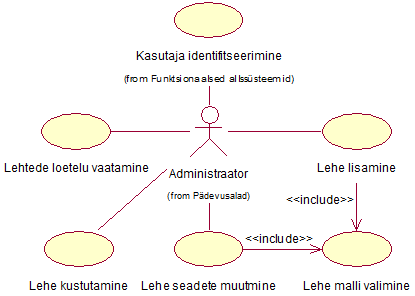
\includegraphics[bb=0 0 483 304,scale=1]{./diagrams/pages-subsystem-use-case-digram.png}
\caption{Lehtede funktsionaalse allsüsteemi kasutusjuhtude eskiismudel}
\end{center}
\end{figure}

\subsection{Regioonide funktsionaalne allsüsteem}
\subsubsection{Eesmärgid}
\begin{itemize}
\item Võimaldada administraatoril saada ülevaade lehel olevatest regioonidest.
\item Võimaldada administraatoril luua navigatsiooni tüüpi regioone.
\item Võimaldada administraatoril luua HTML tüüpi regioone.
\item Võimaldada administraatoril luua raporti tüüpi regioone.
\item Võimaldada administraatoril luua vormi tüüpi regioone.
\item Võimaldada administraatoril muuta olemasolevaid regioone.
\item Võimaldada administraatoril kustutada olemasolevaid regioone.
\end{itemize}
\subsubsection{Allsüsteemi poolt kasutatavad registrid}
Allsüsteem teenindab regioonide registrit.\par
Allsüsteem kasutab mallide registrit, navigatsioonide registrit, andmebaasiobjektide registrit.
\subsubsection{Allsüsteemi kasutusjuhtude eskiismudel}
Järgnevalt on esitatud regioonide funktsionaalse allsüsteemi kasutusjuhtude eskiismudel ja seal esitatud tekstikirjeldused kõrgtaseme formaadis.
\begin{figure}[H]
\begin{center}
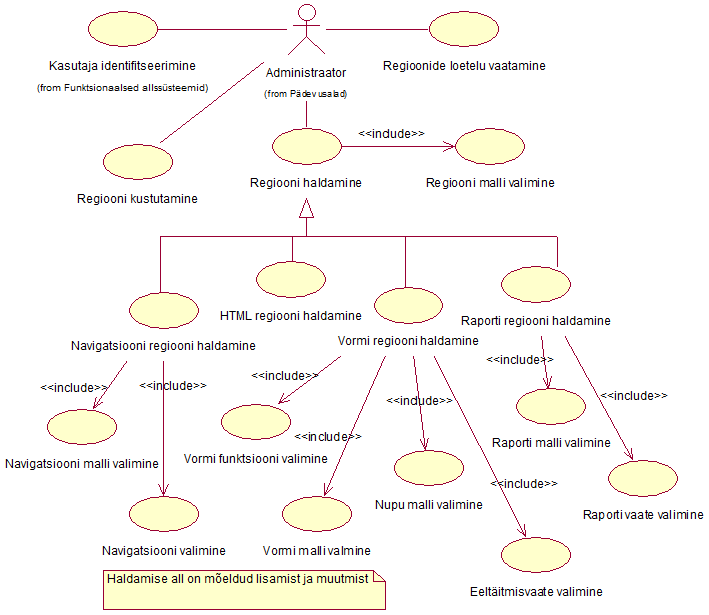
\includegraphics[bb=0 0 709 615,scale=0.85]{./diagrams/regions-subsystem-use-case-digram.png}
\caption{Regioonide funktsionaalse allsüsteemi kasutusjuhtude eskiismudel}
\end{center}
\end{figure}

\subsection{Navigatsioonide funktsionaalne allsüsteem}
\subsubsection{Eesmärgid}
\begin{itemize}
\item Võimaldada administraatoril saada ülevaade rakendusele kuuluvatest navigatsioonidest.
\item Võimaldada administraatoril luua uusi navigatsioone.
\item Võimaldada administraatoril muuta olemasolevate navigatsioonide seadeid.
\item Võimaldada administraatoril kustutada olemasolevaid navigatsioone.
\item Võimaldada administraatoril lisada olemasoleva navigatsiooni alla navigatsioonipunkte.
\item Võimaldada administraatoril muuta olemasolevaid navigatsioonipunkte.
\item Võimaldada administraatoril kustutada olemas olevaid navigatsioonipunkte.
\end{itemize}
\subsubsection{Allsüsteemi poolt kasutatavad registrid}
Allsüsteem teenindab navigatsioonide registrit.\par
Allsüsteem kasutab lehtede registrit.
\subsubsection{Allsüsteemi kasutusjuhtude eskiismudel}
Järgnevalt on esitatud navigatsioonide funktsionaalse allsüsteemi kasutusjuhtude eskiismudel ja seal esitatud tekstikirjeldused kõrgtaseme formaadis.
\begin{figure}[H]
\begin{center}
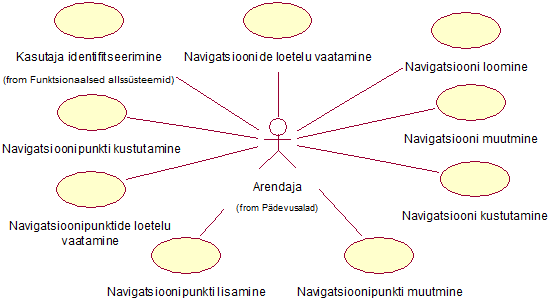
\includegraphics[bb=0 0 582 434,scale=1]{./diagrams/navigations-subsystem-use-case-digram.png}
\caption{Navigatsioonide funktsionaalse allsüsteemi kasutusjuhtude eskiismudel}
\end{center}
\end{figure}

\subsection{Mittefunktsionaalsed nõuded}
\begin{table}[H]%[!htb]
\begin{center}
\begin{tabular}{|p{4cm}|p{11cm}|}
\hline
\rowcolor{rowgray}
Tüüp & Nõude kirjeldus \\ \hline

Serveri tarkvara & Andmete hoidmiseks peab kasutama andmebaasisüsteemi PostgreSQL 9.4 või uuemat. Rakendus tuleb luua kasutades PHP 5.5.0 või uuemat. \\ \hline

Keel & Süsteemi kasutajaliides peab olema ingliskeelne. \\ \hline

Kasutajaliides & Kasutajaliides peab olema veebipõhine ning arvestama erinevate resolutsioonidega. \\ \hline
 
Toetatud veebibrauserid & 
\begin{itemize}
\item Microsoft Internet Explorer 11 või uuem.
\item Mozilla Firefox 43 või uuem.
\item Google Chrome 49 või uuem.
\end{itemize}
 \\ \hline

Andmebaasioperatsioonide töökoorus & Andmebaasioperatsioonid peavad süsteemil aega võtma alla 5 sekundi. \\ \hline

\end{tabular}
\caption{Mittefunktsionaalsed nõuded}
\label{mittefunktsionaalsed_nõuded}
\end{center}
\end{table}


\section{Andmebaasi disain}
\section{Kasutajaliidese disain}
\section{Rakenduse disain}
\section{Näide}

%-------------------------------KOKKUVÕTE---------------------------
\section{Kokkuvõte}
Kokkuvõte

\pagebreak

\section{Summary}
Kokkuvõte

\pagebreak

%------------------------------KASUTATUD KIRJANDUS-----------------------------------
\addcontentsline{toc}{section}{Kasutatud kirjandus}
\bibliographystyle{plain}
\bibliography{pgapex}

\pagebreak

%-----------------------------LISAD--------------------------------
\section*{Lisa 1 - [Pealkiri]}
\addcontentsline{toc}{section}{Lisa 1}

\end{document}
